

\setcounter{exo}{0}
\vfill
\begin{correction}
\begin{multicols}{2}
%
%\exo{}
%
%\begin{enumerate}
%	\item $2z$
%	\item $3z$
%	\item $\frac{z}{2}$
%	\item $7z$
%	\item $5z+2z=7z$
%	\item $2(5+z)$
%\end{enumerate}

%% for i in range(0,61,20) 
\exo{ - Version <<i / 20 +1>>}

Programme 1 : $<<nZ[1+i]>> x <<terme(nZ[2+i])>>$\\
Programme 2 : $(x <<terme(-nZ[3+i])>>)\times <<facteur(nZ[4+i])>>= <<nZ[4+i]>>  x  << terme(- nZ[4+i] * nZ[3+i] ) >> $\\
Programme 3 : $( <<nZ[5+i]>> x <<terme(-nZ[6+i])>> )\times 2= <<2* nZ[5+i]>> x <<terme(-2*nZ[6+i])>>$

%% endfor

%% for i in range(0,61,20) 
\exo{ - Version <<i / 20 +1>>}

%Simplifier les expressions suivantes.

%\begin{multicols}{2}
$A=(<<n[1+i]>>  <<terme(m[1+i])>>) x=<<n[1+i] +m[1+i]>> x$\\
$B=<<mZ[2+i]>> \times x\times x=<<mZ[2+i]>> x^2$\\
$C=(<<nZ[7+i]>> <<terme(nZ[8+i])>>) \times x=<<nZ[7+i] + nZ[8+i]>>  x$\\
$D=<<nZ[7+i]>>\times <<facteur(nZ[8+i])>>\times x\times x=<<nZ[7+i]* nZ[8+i]>> x^2$\\
$E= <<nZ[9+i]>>  x <<terme(nZ[12+i])>> x <<terme(nZ[10+i])>>\times <<facteur(nZ[11+i])>> = (<<nZ[9+i]>>  <<terme(nZ[12+i])>>) x <<terme(nZ[10+i] * nZ[11+i])>> = <<nZ[9+i] + nZ[12+i]>> x <<terme(nZ[10+i] * nZ[11+i])>> $\\
$F=<<nZ[13+i]>> \times (<<nZ[14+i]>>y <<terme(nZ[15+i])>>)  =<<nZ[13+i]>> \times <<facteur(nZ[14+i])>>y <<terme(nZ[13+i])>> \times <<facteur(nZ[15+i])>>
 =<<nZ[13+i]* nZ[14+i]>>y <<terme(nZ[13+i]*nZ[15+i])>> $\\
$G=<<N2[1+i]>> a^2+a\times (<<N2[2+i]>>+ <<N3[1+i]>>)=<<N2[1+i]>> a^2+<<N2[2+i] + N3[1+i]>>a$\\
$H= (<<nZ[17+i]>> <<terme(nZ[18+i])>>)x = <<nZ[17+i] + nZ[18+i]>>x$
%\end{multicols}
%% endfor


%% for i in range(0,61,20) 
\exo{ - Version <<i / 20 +1>>}
%Développer et réduire les expressions suivantes.
%\begin{multicols}{2}
$A=  <<mZ[12+i]>> (x  <<terme(mZ[13+i])>>)=  <<mZ[12+i]>> x <<terme(mZ[12+i])>> \times <<facteur(mZ[13+i])>>=  <<mZ[12+i]>> x <<terme(mZ[12+i] * mZ[13+i])>>$\\
$B= <<mZ[11+i]>> ( <<mZ[10+i]>> x    <<terme(mZ[9+i])>>)= <<mZ[11+i]>> \times <<facteur(mZ[10+i])>> x  <<terme(mZ[11+i])>> \times  <<facteur(mZ[9+i])>>= <<mZ[11+i] * mZ[10+i]>> x  <<terme(mZ[11+i]*mZ[9+i])>>$\\
$C=y( <<mZ[7+i]>>  <<terme(mZ[8+i])>> y)=y \times <<facteur(mZ[7+i])>> + y \times <<mZ[8+i]>> y=<<mZ[7+i]>> y + <<mZ[8+i]>> y^2$\\
$D= <<mZ[6+i]>>  t(  <<mZ[5+i]>> t <<terme(mZ[4+i])>>)= <<mZ[6+i]>>  t \times <<facteur(mZ[5+i])>> t <<terme(mZ[6+i])>>  t \times <<facteur(mZ[4+i])>> = <<mZ[6+i]*mZ[5+i]>>  t^2  <<terme(mZ[6+i]*mZ[4+i])>>  t  $
%\end{multicols}
%% endfor


%% for i in range(0,61,20) 
\exo{ - Version <<i / 20 +1>>}

%Factoriser les expressions suivantes.

%\begin{multicols}{2}
$E=  <<N[5+i]>>x \times <<n[1+i]>>   <<terme(S[1+i])>> \times  <<n[1+i]>> =   (<<N[5+i]>>  x  <<terme(S[1+i])>> ) \times <<n[1+i]>> $\\
$F=  <<S[6+i] *n[6+i]*n[2+i]>>  x  <<terme(S[2+i]*n[2+i])>>  x=  (<<S[6+i] *n[6+i]*n[2+i]>>   <<terme(S[2+i]*n[2+i])>> ) \times  x=  <<S[6+i] *n[6+i]*n[2+i]+S[2+i]*n[2+i]>>  x$\\
$G=  <<S[7+i] *N[7+i] * n[3+i]>> \times  x  <<terme(S[3+i] * n[3+i])>> x\times x=  (<<S[7+i] *N[7+i] * n[3+i]>>   <<terme(S[3+i] * n[3+i])>> x) \times  x$\\
$H=  <<S[8+i] *n[8+i] >> x^2  <<terme(S[4+i] *n[4+i] )>> x^2=  (<<S[8+i] *n[8+i] >> <<terme(S[4+i] *n[4+i] )>>) x^2=  <<S[8+i] *n[8+i] + S[4+i] *n[4+i] >> x^2$
%\end{multicols}
%% endfor

\end{multicols}

\exon{}

\begin{minipage}{0.4\linewidth}
	\begin{center}
	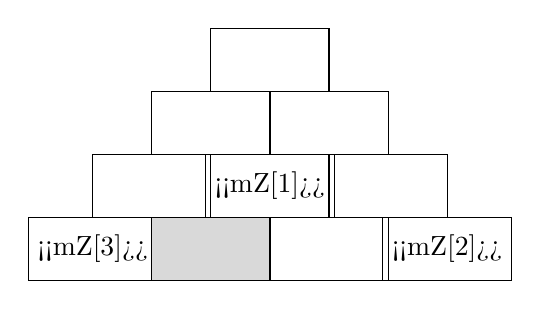
\begin{tikzpicture}
		\tikzstyle{brique}=[minimum width=1.5cm, minimum height=0.8cm,draw]
		\tikzstyle{brique_grise}=[minimum width=1.5cm, minimum height=0.8cm,draw,fill=gray!30]
		\node[brique] at (0,0) {  <<mZ[3]>> }; % gauche
		\node[brique_grise] at (1.5,0) {};
		\node[brique] at (3,0) {};
		\node[brique] at (4.5,0) { <<mZ[2]>> };  % droite
		\node[brique] at (.75,.8) {};
		\node[brique] at (2.25,.8) {  <<mZ[1]>> };  % milieu bas
		\node[brique] at (3.75,.8) {};
		\node[brique] at (1.5,1.6) {};
		\node[brique] at (3,1.6) {};
		\node[brique] at (2.25,2.4) {};
	\end{tikzpicture} 	
\end{center}
\end{minipage}
\begin{minipage}{0.2\linewidth}
%Pour compléter cette pyramide, le nombre situé dans une case est la somme des deux nombres situés en dessous de lui.

\begin{enumerate}
	\item Fait à gauche.
	\item On peut mettre un nombre $x$ quelconque dans la case grise, on trouve toujours <<mZ[3] + mZ[2] + 3*mZ[1]>> dans la case la plus haute. Voir à droite.
\end{enumerate}
\end{minipage}
\begin{minipage}{0.4\linewidth}
	\begin{center}
	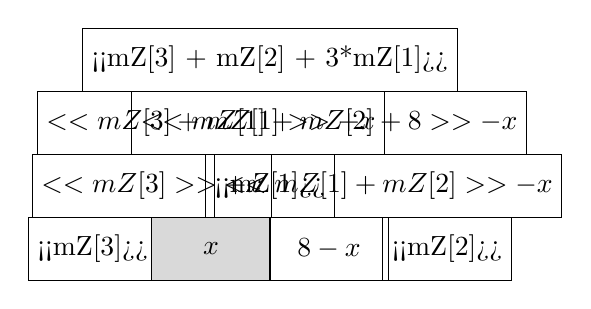
\begin{tikzpicture}
		\tikzstyle{brique}=[minimum width=1.5cm, minimum height=0.8cm,draw]
		\tikzstyle{brique_grise}=[minimum width=1.5cm, minimum height=0.8cm,draw,fill=gray!30]
		\node[brique] at (0,0) {  <<mZ[3]>> }; % gauche
		\node[brique_grise] at (1.5,0) {$x$};
		\node[brique] at (3,0) {$8-x$};
		\node[brique] at (4.5,0) { <<mZ[2]>> };  % droite
		\node[brique] at (.75,.8) {$<<mZ[3]>>+x$};
		\node[brique] at (2.25,.8) {  <<mZ[1]>> };  % milieu bas
		\node[brique] at (3.75,.8) {$<<mZ[1]+mZ[2]>>-x$};
		\node[brique] at (1.5,1.6) {$<<mZ[3]+mZ[1]>>+x$};
		\node[brique] at (3,1.6) {$<<mZ[1]+mZ[2]+8>>-x$};
		\node[brique] at (2.25,2.4) {<<mZ[3] + mZ[2] + 3*mZ[1]>>};
	\end{tikzpicture} 	
\end{center}
\end{minipage}


\end{correction}
